\newcommand{\seccion}{SECUNDARIA INCORPORADA A LA SEG }
\newcommand{\descripcion}{Examen Bimestral, Tercer Bimestre}
\newcommand{\grado}{Primero de secundaria}
\newcommand{\ciclo}{Ciclo escolar: 2015--2016}
\newcommand{\papel}{legalpaper} %letter, legalpaper ...
\newcommand{\fecha}{1 de marzo de 2016}
% \author{Ing. Arturo Canedo \\ M. en C. Reinaldo Zapata}
\author{M. en C. Reinaldo Zapata}

\documentclass[11pt]{article}
\usepackage[\papel,showframe]{geometry}

\title{\flushleft \seccion \\ \descripcion \\  \grado \\ \ciclo}

\newcommand\BackgroundLogo{
\put(160,365){
\parbox[b][\paperheight]{\paperwidth}{%
\vfill
\centering
\includegraphics[width=5cm,height=2.5cm,keepaspectratio]{/Users/reinaldo/Documents/clases/jassa/logo}%
\vfill
}}}


\hyphenation{con-ti-nua-ción}

\usepackage{enumitem}
\usepackage[T1]{fontenc} %fuentes
\usepackage{lmodern} %fuente mejorada
\usepackage[spanish]{babel}
\decimalpoint
\usepackage{fullpage}
\usepackage{multicol}
\usepackage{graphicx}
\usepackage{eso-pic}
\usepackage{multirow}
\usepackage{subfigure}
\usepackage{tikz}


%Modificación del formato de las ecuaciones y el numerado de las mismas
\usepackage[leqno,fleqn]{amsmath}
\makeatletter
  \def\tagform@#1{\maketag@@@{#1\@@italiccorr}}
\makeatother
\renewcommand{\theequation}{\fbox{\textbf{\arabic{equation}}}}


\begin{document}
\AddToShipoutPicture*{\BackgroundLogo}
\ClearShipoutPicture
\date{\fecha}
\maketitle
% \thispagestyle{empty}


Nombre del alumno:\,\line(1,0){244}\,.\hspace*{.2cm} \hfill Aciertos:
$\dfrac{\qquad \qquad}{50}$.

\vspace{3mm}
\indent Primero de secundaria, grupo:\,\line(1,0){35}\,. No. de
lista:\,\line(1,0){35}\,.

\vspace{5mm}

El prop\'osito de todo examen es poner a prueba los conocimientos de cada alumno
para calificar as\'i su desempe\~no y aprendizaje. Contesta correctamente, en
cada secci\'on, tantos reactivos como te sea posible. Todas y cada una de las
operaciones deber\'as escribirlas en esta hoja donde se imprimi\'o el examen y
los resultados finales deber\'an estar escritos con tinta.

\section{Geometr\'ia} % (fold)
\label{sec:geometr'ia}

Usando fracciones, calcula el \'area de un tri\'angulo cuya base mide
$b=\frac{5}{3}$\,m y su altura mide $h=1.5$\,m. Para ello convierte primero la
altura a fracci\'on. \hfill(valor: 4 aciertos.)

\vspace{4cm}
El Pent\'agono, edificio del Departamento de Defensa de los Estados Unidos, es
uno gran edificio de oficinas en el que trabajan cerca de 23,000 personas. Una
fotograf\'ia del mismo se muestra a continuaci\'on. Se sabe que su longitud
lateral es $\ell=281$\,m y su apotema mide $a=193.3$\,m. Calcula el \'area de
dicho edificio utilizando decimales. \hfill(valor: 5 aciertos.)

\begin{figure}[h!]
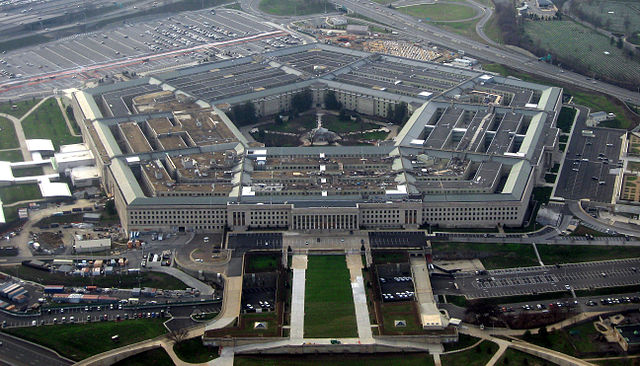
\includegraphics[width=0.35\linewidth]{pentagono.jpg}
\label{fig:pentagono}
\end{figure}

Cierta compa\~nia de contratistas le paga a los alba\~niles \$115.00 por cada
metro cuadrado de pared que construyen. Uno de los obreros construye una barda
rectangular cuya base mide $b=6$\,m y altura $h=2.5$\,m. ?`Cu\'al deber\'a ser la
paga que reciba por dicho trabajo? \hfill(valor: 4 aciertos.)

% section geometr'ia (end)

\newpage
Traza una l\'inea horizontal de 3\,cm y un \'angulo de $45^{\circ}$. Traza sus
correspondientes mediatriz y bisectriz. \hfill(valor: 2 aciertos.)

\vspace{4cm}
\section{Proporcionalidad} % (fold)
\label{sec:proporcionalidad}

El profesor de matem\'aticas viaja en su autom\'ovil recorriendo en promedio
una distancia de 120\,Km cada hora. ?`Cu\'anto tiempo le tomar\'a llegar a la
ciudad de Guanajuato si la distancia es de 64\,Km? \hfill(valor: 3 aciertos.)

\vspace{3.5cm}
?`Cu\'anto es el 25\% de 350? \hfill(valor: 2 aciertos.)

\vspace{3.5cm}
\section{probabilidad y estad\'istica} % (fold)
\label{sec:probabilidad_y_estad'istica}

% section proporcionalidad (end)

A continuaci\'on se presenta un conjunt de n\'umeros. Calcula su media, moda y 
mediana.

17, 5, 5, 11, 17, 13. \hfill(valor: 4 aciertos.)

\vspace{5cm}
Se tiene una bolsa con 20 caramelos de colores de los cuales 10 (50\%) son de
color rojo, 6 (30\%) verdes y 4 (20\%) de color amarillo. Si se sacan caramelos
al azar, de manera similar a como se hizo en clase, ?`Cu\'al es el color que
tiene m\'as probabilidades de salir? Explica el motivo. 

\hfill(valor: 4 aciertos.)

\newpage
Si hacemos el experimento anterior sacando 10 dulces, ?`se cumplir\'a
forzosamente que 3 dulces sean rojos, 3 verdes y 4 amarillos? Explica la
situaci\'on con tus palabras. \hfill(valor: 3 aciertos.)

% section probabilidad_y_estad'istica (end)

\vspace{2cm}
\section{Introducci\'on al \'Algebra} % (fold)
\label{sec:introducci'on_al_'algebra}

Completa la tabla que se muestra a continuaci\'on separando las expresiones
algebraicas en sus respectivos componentes. \hfill(valor: 8 aciertos.)

\begin{center}
\bgroup
\def\arraystretch{2}
\begin{tabular}{|c|c|c|c|}
\hline
Expresi\'on & Coeficiente & Literal(es) & Exponente(s)  \\ \hline 
$3x^2$ &&&\\ \hline
$b^2c^4x^6$ &&&\\ \hline
$17ax^2y^3$ &&&\\ \hline
$d^2we^3x$ &&&\\ \hline
\end{tabular}
\egroup
\end{center}

\vspace{5mm}
Resuelve las siguientes ecuaciones: \hfill(valor: 6 aciertos.)

\vspace{-8mm}
\begin{multicols}{2}

\begin{equation*}
7x + 3 = 38
\end{equation*}

\begin{equation*}
6x - 3 = 1
\end{equation*}

\end{multicols}

\vspace{5cm}
Cinco veces un n\'umero menos 10 da como resultado 40. ?`Cu\'al es ese n\'umero?
Plantea la ecuaci\'on que describe este problema y resu\'elvela. \hfill(valor: 5
aciertos.)


% section introducci'on_al_'algebra (end)



\end{document}






